\documentclass[journal,compsoc, 10pt, draftclsnofoot, onecolumn]{IEEEtran}

\usepackage{graphicx}
\usepackage{amssymb}
\usepackage{amsmath}
\usepackage{amsthm}
\usepackage{tabularx}
\usepackage{graphicx}

\newcommand{\subparagraph}{}
\usepackage{titlesec}

\usepackage{alltt}
\usepackage{float}
\usepackage{color}
\usepackage{url}

\usepackage{balance}
\usepackage[TABBOTCAP, tight]{subfigure}
\usepackage{enumitem}
\usepackage{pstricks, pst-node}

\usepackage{cite}
\usepackage{listings}
\usepackage{placeins}

\usepackage[margin=0.75in]{geometry}
\geometry{textheight=8.5in, textwidth=6in}

\renewcommand{\sfdefault}{\sfdefault}

\newlength\tindent
\setlength{\tindent}{\parindent}
\setlength{\parindent}{0pt}
\renewcommand{\indent}{\hspace*{\tindent}}

\newcommand{\cred}[1]{{\color{red}#1}}
\newcommand{\cblue}[1]{{\color{blue}#1}}

\newcommand{\namesigdate}[2][6cm]{%
  \begin{tabular}{@{}p{#1}@{}}
    #2 \\[0.5\normalbaselineskip] \hrule \\[0.pt]
    {\small \textit{Signature}} \\[0.5\normalbaselineskip] \hrule \\[0pt]
    {\small \textit{Date}}
  \end{tabular}
}


\usepackage{hyperref}
\usepackage{geometry}

\lstset{
language=C,
basicstyle=\ttfamily,
commentstyle=\color{blue},
keywordstyle=\color{green},
numberstyle=\color{red},
stringstyle=\color{orange}
}

\def\nameD{Devin Foulger}
\def\nameH{Hector Trujillo}
\def\nameB{Bryan Liauw}

\usepackage{fancyvrb}
\usepackage{color}
\usepackage[latin1]{inputenc}


\makeatletter
\def\PY@reset{\let\PY@it=\relax \let\PY@bf=\relax%
    \let\PY@ul=\relax \let\PY@tc=\relax%
    \let\PY@bc=\relax \let\PY@ff=\relax}
\def\PY@tok#1{\csname PY@tok@#1\endcsname}
\def\PY@toks#1+{\ifx\relax#1\empty\else%
    \PY@tok{#1}\expandafter\PY@toks\fi}
\def\PY@do#1{\PY@bc{\PY@tc{\PY@ul{%
    \PY@it{\PY@bf{\PY@ff{#1}}}}}}}
\def\PY#1#2{\PY@reset\PY@toks#1+\relax+\PY@do{#2}}

\expandafter\def\csname PY@tok@gd\endcsname{\def\PY@tc##1{\textcolor[rgb]{0.63,0.00,0.00}{##1}}}
\expandafter\def\csname PY@tok@gu\endcsname{\let\PY@bf=\textbf\def\PY@tc##1{\textcolor[rgb]{0.50,0.00,0.50}{##1}}}
\expandafter\def\csname PY@tok@gt\endcsname{\def\PY@tc##1{\textcolor[rgb]{0.00,0.25,0.82}{##1}}}
\expandafter\def\csname PY@tok@gs\endcsname{\let\PY@bf=\textbf}
\expandafter\def\csname PY@tok@gr\endcsname{\def\PY@tc##1{\textcolor[rgb]{1.00,0.00,0.00}{##1}}}
\expandafter\def\csname PY@tok@cm\endcsname{\let\PY@it=\textit\def\PY@tc##1{\textcolor[rgb]{0.25,0.50,0.50}{##1}}}
\expandafter\def\csname PY@tok@vg\endcsname{\def\PY@tc##1{\textcolor[rgb]{0.10,0.09,0.49}{##1}}}
\expandafter\def\csname PY@tok@m\endcsname{\def\PY@tc##1{\textcolor[rgb]{0.40,0.40,0.40}{##1}}}
\expandafter\def\csname PY@tok@mh\endcsname{\def\PY@tc##1{\textcolor[rgb]{0.40,0.40,0.40}{##1}}}
\expandafter\def\csname PY@tok@go\endcsname{\def\PY@tc##1{\textcolor[rgb]{0.50,0.50,0.50}{##1}}}
\expandafter\def\csname PY@tok@ge\endcsname{\let\PY@it=\textit}
\expandafter\def\csname PY@tok@vc\endcsname{\def\PY@tc##1{\textcolor[rgb]{0.10,0.09,0.49}{##1}}}
\expandafter\def\csname PY@tok@il\endcsname{\def\PY@tc##1{\textcolor[rgb]{0.40,0.40,0.40}{##1}}}
\expandafter\def\csname PY@tok@cs\endcsname{\let\PY@it=\textit\def\PY@tc##1{\textcolor[rgb]{0.25,0.50,0.50}{##1}}}
\expandafter\def\csname PY@tok@cp\endcsname{\def\PY@tc##1{\textcolor[rgb]{0.74,0.48,0.00}{##1}}}
\expandafter\def\csname PY@tok@gi\endcsname{\def\PY@tc##1{\textcolor[rgb]{0.00,0.63,0.00}{##1}}}
\expandafter\def\csname PY@tok@gh\endcsname{\let\PY@bf=\textbf\def\PY@tc##1{\textcolor[rgb]{0.00,0.00,0.50}{##1}}}
\expandafter\def\csname PY@tok@ni\endcsname{\let\PY@bf=\textbf\def\PY@tc##1{\textcolor[rgb]{0.60,0.60,0.60}{##1}}}
\expandafter\def\csname PY@tok@nl\endcsname{\def\PY@tc##1{\textcolor[rgb]{0.63,0.63,0.00}{##1}}}
\expandafter\def\csname PY@tok@nn\endcsname{\let\PY@bf=\textbf\def\PY@tc##1{\textcolor[rgb]{0.00,0.00,1.00}{##1}}}
\expandafter\def\csname PY@tok@no\endcsname{\def\PY@tc##1{\textcolor[rgb]{0.53,0.00,0.00}{##1}}}
\expandafter\def\csname PY@tok@na\endcsname{\def\PY@tc##1{\textcolor[rgb]{0.49,0.56,0.16}{##1}}}
\expandafter\def\csname PY@tok@nb\endcsname{\def\PY@tc##1{\textcolor[rgb]{0.00,0.50,0.00}{##1}}}
\expandafter\def\csname PY@tok@nc\endcsname{\let\PY@bf=\textbf\def\PY@tc##1{\textcolor[rgb]{0.00,0.00,1.00}{##1}}}
\expandafter\def\csname PY@tok@nd\endcsname{\def\PY@tc##1{\textcolor[rgb]{0.67,0.13,1.00}{##1}}}
\expandafter\def\csname PY@tok@ne\endcsname{\let\PY@bf=\textbf\def\PY@tc##1{\textcolor[rgb]{0.82,0.25,0.23}{##1}}}
\expandafter\def\csname PY@tok@nf\endcsname{\def\PY@tc##1{\textcolor[rgb]{0.00,0.00,1.00}{##1}}}
\expandafter\def\csname PY@tok@si\endcsname{\let\PY@bf=\textbf\def\PY@tc##1{\textcolor[rgb]{0.73,0.40,0.53}{##1}}}
\expandafter\def\csname PY@tok@s2\endcsname{\def\PY@tc##1{\textcolor[rgb]{0.73,0.13,0.13}{##1}}}
\expandafter\def\csname PY@tok@vi\endcsname{\def\PY@tc##1{\textcolor[rgb]{0.10,0.09,0.49}{##1}}}
\expandafter\def\csname PY@tok@nt\endcsname{\let\PY@bf=\textbf\def\PY@tc##1{\textcolor[rgb]{0.00,0.50,0.00}{##1}}}
\expandafter\def\csname PY@tok@nv\endcsname{\def\PY@tc##1{\textcolor[rgb]{0.10,0.09,0.49}{##1}}}
\expandafter\def\csname PY@tok@s1\endcsname{\def\PY@tc##1{\textcolor[rgb]{0.73,0.13,0.13}{##1}}}
\expandafter\def\csname PY@tok@sh\endcsname{\def\PY@tc##1{\textcolor[rgb]{0.73,0.13,0.13}{##1}}}
\expandafter\def\csname PY@tok@sc\endcsname{\def\PY@tc##1{\textcolor[rgb]{0.73,0.13,0.13}{##1}}}
\expandafter\def\csname PY@tok@sx\endcsname{\def\PY@tc##1{\textcolor[rgb]{0.00,0.50,0.00}{##1}}}
\expandafter\def\csname PY@tok@bp\endcsname{\def\PY@tc##1{\textcolor[rgb]{0.00,0.50,0.00}{##1}}}
\expandafter\def\csname PY@tok@c1\endcsname{\let\PY@it=\textit\def\PY@tc##1{\textcolor[rgb]{0.25,0.50,0.50}{##1}}}
\expandafter\def\csname PY@tok@kc\endcsname{\let\PY@bf=\textbf\def\PY@tc##1{\textcolor[rgb]{0.00,0.50,0.00}{##1}}}
\expandafter\def\csname PY@tok@c\endcsname{\let\PY@it=\textit\def\PY@tc##1{\textcolor[rgb]{0.25,0.50,0.50}{##1}}}
\expandafter\def\csname PY@tok@mf\endcsname{\def\PY@tc##1{\textcolor[rgb]{0.40,0.40,0.40}{##1}}}
\expandafter\def\csname PY@tok@err\endcsname{\def\PY@bc##1{\setlength{\fboxsep}{0pt}\fcolorbox[rgb]{1.00,0.00,0.00}{1,1,1}{\strut ##1}}}
\expandafter\def\csname PY@tok@kd\endcsname{\let\PY@bf=\textbf\def\PY@tc##1{\textcolor[rgb]{0.00,0.50,0.00}{##1}}}
\expandafter\def\csname PY@tok@ss\endcsname{\def\PY@tc##1{\textcolor[rgb]{0.10,0.09,0.49}{##1}}}
\expandafter\def\csname PY@tok@sr\endcsname{\def\PY@tc##1{\textcolor[rgb]{0.73,0.40,0.53}{##1}}}
\expandafter\def\csname PY@tok@mo\endcsname{\def\PY@tc##1{\textcolor[rgb]{0.40,0.40,0.40}{##1}}}
\expandafter\def\csname PY@tok@kn\endcsname{\let\PY@bf=\textbf\def\PY@tc##1{\textcolor[rgb]{0.00,0.50,0.00}{##1}}}
\expandafter\def\csname PY@tok@mi\endcsname{\def\PY@tc##1{\textcolor[rgb]{0.40,0.40,0.40}{##1}}}
\expandafter\def\csname PY@tok@gp\endcsname{\let\PY@bf=\textbf\def\PY@tc##1{\textcolor[rgb]{0.00,0.00,0.50}{##1}}}
\expandafter\def\csname PY@tok@o\endcsname{\def\PY@tc##1{\textcolor[rgb]{0.40,0.40,0.40}{##1}}}
\expandafter\def\csname PY@tok@kr\endcsname{\let\PY@bf=\textbf\def\PY@tc##1{\textcolor[rgb]{0.00,0.50,0.00}{##1}}}
\expandafter\def\csname PY@tok@s\endcsname{\def\PY@tc##1{\textcolor[rgb]{0.73,0.13,0.13}{##1}}}
\expandafter\def\csname PY@tok@kp\endcsname{\def\PY@tc##1{\textcolor[rgb]{0.00,0.50,0.00}{##1}}}
\expandafter\def\csname PY@tok@w\endcsname{\def\PY@tc##1{\textcolor[rgb]{0.73,0.73,0.73}{##1}}}
\expandafter\def\csname PY@tok@kt\endcsname{\def\PY@tc##1{\textcolor[rgb]{0.69,0.00,0.25}{##1}}}
\expandafter\def\csname PY@tok@ow\endcsname{\let\PY@bf=\textbf\def\PY@tc##1{\textcolor[rgb]{0.67,0.13,1.00}{##1}}}
\expandafter\def\csname PY@tok@sb\endcsname{\def\PY@tc##1{\textcolor[rgb]{0.73,0.13,0.13}{##1}}}
\expandafter\def\csname PY@tok@k\endcsname{\let\PY@bf=\textbf\def\PY@tc##1{\textcolor[rgb]{0.00,0.50,0.00}{##1}}}
\expandafter\def\csname PY@tok@se\endcsname{\let\PY@bf=\textbf\def\PY@tc##1{\textcolor[rgb]{0.73,0.40,0.13}{##1}}}
\expandafter\def\csname PY@tok@sd\endcsname{\let\PY@it=\textit\def\PY@tc##1{\textcolor[rgb]{0.73,0.13,0.13}{##1}}}

\def\PYZbs{\char`\\}
\def\PYZus{\char`\_}
\def\PYZob{\char`\{}
\def\PYZcb{\char`\}}
\def\PYZca{\char`\^}
\def\PYZam{\char`\&}
\def\PYZlt{\char`\<}
\def\PYZgt{\char`\>}
\def\PYZsh{\char`\#}
\def\PYZpc{\char`\%}
\def\PYZdl{\char`\$}
\def\PYZti{\char`\~}
% for compatibility with earlier versions
\def\PYZat{@}
\def\PYZlb{[}
\def\PYZrb{]}
\makeatother


\hypersetup {
        colorlinks = true,
        urlcolor = black,
        linkcolor = black,
        pdfauthor = {\nameD\nameH\nameB},
        pdfkeywords = {},
        pdfsubject = {},
        pdfpagemode = UseNone
}

\titleformat{\section}
	{\normalfont\fontsize{15}{10}\bfseries}{\thesection}{1em}{}
\titleformat{\subsection}
	{\normalfont\fontsize{12}{15}\bfseries}{\thesubsection}{1em}{}
\titleformat{\subsubsection}
	{\normalfont\fontsize{12}{15}\bfseries}{\thesubsubsection}{1em}{}

\begin{document}

\title{\vspace{20em}Design Document \\{\vspace{-1ex}\huge UniversityGear} \\
{\large \today}}
\author{\vspace{10ex}Devin Foulger \\{\vspace{-1ex}Hector Trujillo}
\\{\vspace{-1ex}Bryan Liauw}}

\begin{titlepage}

\maketitle
\thispagestyle{empty}

\begin{abstract}
This design document will outline and describe the steps we will take to develop 
our application "UniversityGear."  It will talk about the purpose of this 
document as well as many of the different viewpoints. It will also define 
the classes and methods that we will use in our project. 
\end{abstract}

\vspace{2ex}\noindent 
\namesigdate{Luther Boorn} \hfill
\namesigdate{Devin Foulger} \hfill

\vspace{4ex}\noindent
\namesigdate{Hector Trujillo} \hfill
\namesigdate{Brian Liauw} \hfill

\end{titlepage}

\tableofcontents


\section{Introduction}
\subsection{Scope}
The application that is going to be developed will be for Android devices, 
specifically for N and M OS. It will allow users to purchase college merchandise
 via eBay's large collection of items. The user will be able to search for items
 from different colleges or by specific search criteria. The project will begin 
development in December, 2016 and end in May, 2017.

\subsection{Purpose}
The purpose of this design document is to outline how the application will be 
structured to satisfy the requirements we have set. It will go into depth about 
the design details of our software.

\subsection{Intended Audience}
The intended audience is for the team "4Credit" and their client. It is also for
 the professors of the senior capstone class at Oregon State University.

\section{Definitions}

\begin{table}[!h]
\centering
\caption{Definitions}
\label{my-label}
\begin{tabularx}{\textwidth}{l|X}
\hline
\textbf{Term}               & \textbf{Definition}                                                                                                           \\ \hline
API                    	      & Application Programming Interface, allows developers to develop applications that connect to eBay's large inventory of items. \\ \hline                                                           \\ \hline
Vendors               	      & Individuals or companies that sell or will sell items on eBay                                                                 \\ \hline
Filters                	      & Search criteria that will allow the user to more easily find the item that they are looking for.                              \\ \hline
Third-Party Developers & Individuals outside of eBay that will be using eBay's public APIs to create their own applications.                           \\ \hline
Application            	      & An Android application that uses eBay's public APIs.                                                                          \\ \hline
College Merchandise     & Items such as school supplies for Higher Ed, fan gear, etc...                                                                 \\ \hline
User                   	      & Any one who will be using the Android Application utilizing eBay's APIs.                                                      \\ \hline
Client                 	      & eBay                                                                                                                          \\ \hline
BIN                    	      & Buy It Now                                                                                                                    \\ \hline
N                   	      & Android's new Nougat operating system 
\\ \hline
M                   	      & Android's Marshmallow operating system                                                                                                                   
\\ \hline
MVC                   	      & A design pattern called Model View Controller
\\ \hline
\end{tabularx}
\end{table}
\FloatBarrier


\section{Conceptual model for software design descriptions}
The basic concepts and context of the design document will be explained in this 
section of the document.

\subsection{Software design in context}
An object oriented approach will be taken and we will be using a specific 
design pattern called MVC. This will allow us to maintain some form of a 
separation of concerns. In turn, it will make development much smoother. We will
 also have to keep track of an API layer, as we will be using eBay's new APIs. 
It is imperative that our application also works on the M and N Android 
operating systems.

\subsection{Software design descriptions within the life cycle}
\subsubsection{Influences on design document preparation}
The software requirements specification (SRS) plays a large role in influencing 
the design document. This is because the SRS defines all of the functional and 
interface requirements for the successful completion of the project.

\subsubsection{Design verification and design role in validation}
Test cases will be developed simultaneously to development phase. This will 
allow us to validate that our application is successfully working as expected. 
The last step of validation we will complete if our application successfully 
met the requirements defined in the SRS.


\section{Design description information content}
This section of the design document will identify how the application will be 
implemented and designed. 

\subsection{Design document identification}

\subsection{Design stakeholders and their concerns}
The stakeholders of the project our the developers and their clients. The 
biggest concern is that the product will meet all of the requirements specified 
in the SRS. The application must also contain design that is described in this 
document. 

\subsection{Design views}
We will be using different processes for representing diagrams. We will be using
 UML for describing our functions and classes.

\subsection{Design viewpoints}
The design viewpoints will be described with a combination of UML diagrams and 
short descriptions. The descriptions could include information regarding the 
context, composition, logical, or interactive viewpoints. Each viewpoint will 
also have a specific name.

\subsection{Design elements}
There are a lot of design attributes we will be discussing in our document. Our 
design entities will consist of the APIs and classes that we will be using to 
accomplish our goals. Each entity will have a name, a type, and a purpose. The 
name attribute is simply the name of the element or entity. The type attributes 
will consist of what kind of class or API we will be using. The purpose attribute 
is to give a description as to why an element might exist. Last, an author 
attribute will be used to identify which designer will be responsible for the 
element.

\subsection{Design rationale}
It is important that our application performs well on the N and M Android operating 
systems. We will make sure that the application is also easily maintainable 
for future developers. We will also provide documentation of the design process 
so that other developers will understand the structure of the application.


\section{Design viewpoints}
The main design viewpoints will be explained here. The exact viewpoints are the 
context, composition, logical, dependency, interfaction, and algorithm viewpoints.

\subsection{Context viewpoint}
The context viewpoint will document the functionality between the user and the 
application. There are two main functionalities the user should be using: 
searching and purchasing merchandise. This sections serves to define the user 
interaction with the app. It will also talk about the sub functions that will 
be used to facilitate the main functions. \newline

The user of the application will also have to perform other smaller actions in 
order to get the full use. For example, they will have to download the application 
from the Google Play store. From there, they would be required to search for 
something in order to purchase it. They will be searching for specific schools, 
prices, condition of item, and other search criteria. They will then be presented 
with a list of items in which they will be able to select and view that item in 
greater detail. They will also be able to purchase the item and then they will 
need to enter in their name and shipping information. \newline

When viewing an item in greater detail, the user will be given the opportunity 
to purchase the item. They will have to provide the application with some user 
information, such as a credit card number and shipping address. The user will 
also have to provide other information such as the school they are searching 
for, what item they are looking, the price of the item, condition of the item, 
and other filers of that sort.

\subsection{Composition viewpoint}
The application will be divided into three different parts. The first being the 
search feature, which will allow the user to find a specific item. The second 
will be the purchasing feature, which will allow the user to purchase any item 
they have found. Last, the user should be able to view in detail everything 
about the item they have searched for. All these pieces need to be connected 
together and coherently function as one piece. 

\begin{figure}[h]
\centering
\caption{UML Diagram for the for main classes}
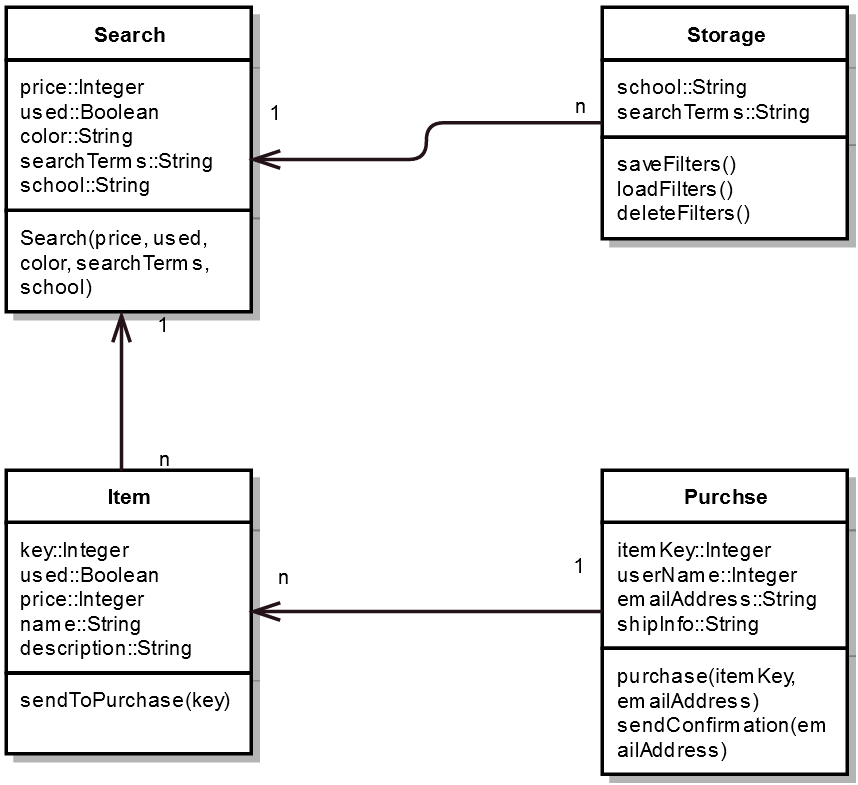
\includegraphics[scale=.65]{projectUML}
\end{figure}
\FloatBarrier

\subsubsection*{Function attribute}
The search class will allow users to search for their items. This class will need 
several variables, which will be passed into a function that calls an API. The 
output will be a list of items that are related to the search criteria provided 
by the user. The author of the search class will be Bryan Liauw. 
The storage class will allow the user to save their search filers 
for later use so they don't have to keep entering the same data each time. This 
requires the same information provided to the search. From there, the class will 
either save, load, or delete this data. Bryan will also be the author of the storage 
class. The item class will be used to hold and 
send the specific item data to the purchase class. Devin Foulger will be the 
author of the item class. The purchase class will allow 
the user to purchase the item that they have selected. It will also send a 
confirmation if the user's purchase has been completed. Devin will also be the 
author of the item class.

\subsubsection*{Subordinates}
The search class will be the default class that will control the application. 
This is because the storage and item classes will depend on the search class 
as you need to search for something in order to save the information and create 
items. The purchase class will depend upon the item class. This is because if 
are no items, then there will be nothing to purchase. In order to purchase 
something, an item must exist. 

\subsection{Logical viewpoint}
Our application will consist of many classes, but they will either be a model or 
a controller. These classes will be the Search class, Purchase class, Item class, 
and the Storage class.

\subsubsection*{The search class}
This class will allow users to search for items that they would like to view or 
purchase. It will share a relationship with the item and storage classes. It 
will have a method for searching that needs the search terms that have been 
provided by the user. The important thing to notice, is the variables provided 
by the user. These variables are the "price", which is a integer. The second is 
the condition of the item, which is called "used" and it is a boolean variable. 
The third variable is the color of the item and is named "color", which it is a 
string value. "searchTerms" is another variable of type string, and is used to 
hold the search values the user provides. The last variable is the "school" and 
is a string. The search method for this class also heavily relies on an API 
called "Browse" which is provided by eBay.

\begin{figure}[h]
\centering
\caption{UML for the search class}
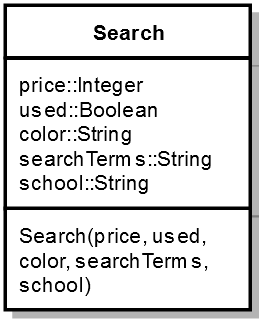
\includegraphics[scale=.9]{searchUML}
\end{figure}
\FloatBarrier

\subsubsection*{The storage class}
This class will be used to save the users search criteria. This is so the user 
will not have to enter in the same information again, considering that they 
will most likely search for the same schools over and over again. It will have 
the ability to save, load, and delete filters. It will also need the information 
provided by the user such as the school and searchTerms. Those variables will be 
provided by the search class. 

\begin{figure}[h]
\centering
\caption{UML for the storage class}
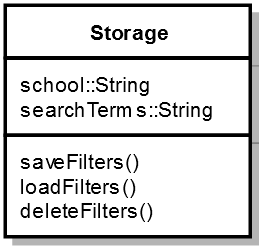
\includegraphics[scale=.9]{storageUML}
\end{figure}
\FloatBarrier

\subsubsection*{The item class}
The item class will hold all the information on a single item. The items will be 
displayed to the user in either a list view or a single item view. The information 
will also be sent to the purchase class so that the user may be able to purchase 
the item. This class heavily relies on what is returned by the search class and 
the Browse API. Every item will have a unique "key", that is an integer value. This 
variable exists so that every item that is in eBay's database has a unique 
identifier. The item will also contain a "used" variable that will be a boolean 
to determine if the item is used. The "price" will be an integer variable that 
determines how expensive the item is. It will also have a "name" and a 
"description" variables,  both will be strings. The "sendToPurchase" method will 
allow users to purchase the item that they have chosen. This means that the key 
will be needed for this transaction to take place. The key will identify which 
item is being purchased. The item class will also need to use the Android JSON 
parser. This is because the returned value from the search from eBay's Order 
API is a JSON file. The JSON parser will need to be able to parse the file for the
correct information.

\begin{figure}[h]
\centering
\caption{UML for the item class}
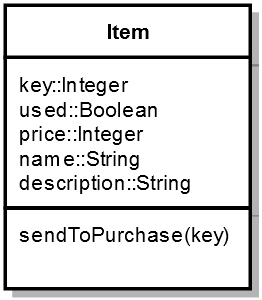
\includegraphics[scale=.9]{itemUML}
\end{figure}
\FloatBarrier

\subsubsection*{The purchase class}
The purchase class will allow the user to purchase the item that they have 
selected. It will need the item key when purchasing an item. It will also notify
the user in some way that they know the purchase has been completed. The first 
variable that is needed is the "itemKey", which is a unique key that identifies 
which item is being purchased. The next variable, is the "userName", which will 
hold the users first and last name. The third variable is a string called 
"emailAddress" that will hold the user provided email address. The last variable, 
"shipInfo" will hold the users shipping address. The "purchase" method will 
require the use of eBay's "Order" API. The purchase method will also need the 
email address. 

\begin{figure}[h]
\centering
\caption{UML for the purchase class}
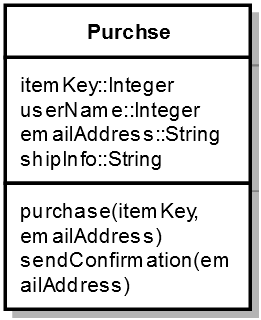
\includegraphics[scale=.9]{purchaseUML}
\end{figure}
\FloatBarrier

\subsection{Dependency viewpoint}
Each class is somewhat dependent on the search class, as it is the basis of 
where everything starts. Item and storage can only exist after something has 
been searched for. The purchase class can only exist if an item exists.

\subsubsection*{Search class dependencies}
The search class does not depend on any other classes in order to function. 
However, it does depend on eBay's Browse API. This API is what will give us the 
ability to search for items.

\subsubsection*{Storage class dependencies}
The storage class depends on the search class. It also depends on what 
information has been provided by the user. The purpose that the storage class 
depends on the search class, is because it needs to save specific information 
such as the school and search terms. The search class also contains the information 
that has been provided by the user, which the storage class will need. 

\subsubsection*{Item class dependencies}
The item class depends on the storage class. This is because it will need 
the information that is returned from the item search. The purpose that this 
class depends on search is because the item will need the information that is 
returned from the search method in the search class. It also depends on the 
Android JSON parser. This is because the returned value from the search method 
will be in a JSON format. The JSON parser API will need to correctly return the 
required information for the item class.

\subsubsection*{Purchase class dependencies}
The purchase class depends on the item class. The class will need the 
information that is in the item class, like the item key. The purpose that this 
class depends on the item class is because purchasing needs the item key. The 
purchase class will also depend on eBay's Oder API. EBay's API will allow the 
class to make its purchase. The API will also need the item key. 

\subsection{Interaction viewpoint}

\subsubsection*{Home Page}
The home page will be a simple design that will include a search bar labeled 
'searchText' and a button 'searchButton' for the user to enter text and 
submit their search. When the user presses the search button, the text within 
the search text field will be passed as a string parameter to the search method.
The user will not be allowed to press the search button without first inputting 
text into the search field. To submit a search from the home page, the user will 
also be allowed to use the search button on the on-screen keyboard. 

\subsubsection*{Multi List View}
This module will proceed the home page, after the user searches for an item. 
After the search module completes its search, it will return a list of data 
structure that contains the search results. The pertinent information in the 
search results will consist of an image of the item for sale, the item name or 
title, and the item price. The DisplayResults module will then take these 
results and present them to the user in a list view. \newline

The image that will be displayed in the list view will be a smaller version of 
the main image. This will be done by the service that will be used by the 
search module. The image size reduction will be necessary to reduce loading 
times and thus performance impacts. \newline

In this same multi list view module, there will be a filter component that will
 allow the users to filter the search results. The users will be able to filter 
the results based on predefined criteria. The currently defined search filters 
include price (Integer), item category (String), or item condition (new or used) 
(Boolean). These details regarding an item will be part of the data that is 
returned by the search module but not displayed to the user until they enter 
the single item view.

\subsubsection*{No Search Results}
If after the user submits their search, or modifies their search criteria to the
 point that there are no search results to display, this module will present a 
message stating that there are no search results and to try a different search, 
or to modify their search criteria. This module will be based off the size of 
the list returned by search.

\subsection{Algorithm viewpoint}
The algorithms viewpoints will describe the different algorithms that we will be
 using to correct users search mistakes. The Levenshtein Distance algorithm that 
we are going to use is going to be attached to the search bar that is in most 
pages of the UI. The algorithm will run every time the users finish typing and 
submitting their search. The algorithm will run regardless whether the keyword 
needs to be corrected or not. The fix will happen if the user has written 
something that is not quite correct; that is, the distance between the intended 
string and the string that user has written does not have a 0 value. Once this 
case happens, we will find the keyword with the minimum distance from the string 
user has written and replace user's keyword with that.

\subsubsection*{Design concerns}
There is a huge concern in terms of resources needed. Since the algorithm is 
going to compare keywords from the user to keywords in the database, this 
means that the algorithm will run once for every words in the database. 
Furthermore, the algorithm itself has a complexity of O n-squared, since the 
number of loops is the string size of one string times the string size of the 
other. This means that the total complexity would be O n-cubed. One way to get 
around this is to find a threshold. Once this threshold is reached, the word 
is considered similar enough. This can reduce a lot of processing time.

\subsubsection*{Processing attribute}
This algorithm will be part of the search method inside the search class. 
Because of this, it will affect only the variables within the class. 
Since we are correcting the users input string, we will use the algorithm to 
manipulate the variable color, school and searchTerms. Fixing price and used 
variable is unnecessary because it does not need to be fixed. The only thing 
we could do to price is find approximate integer to the user’s input, while 
the used variable should not be modified. The algorithm will find the most 
similar string based on the difference in the character in each position. 
This is done by constructing a two-by-two matrix and then filling it with an 
integer based on a certain rule. This rule will measure the differences 
between the characters in each string and assign an integer to determine how 
different it is. As previously mentioned, the loop happens every time user 
enters a keyword. Once the keyword is entered, the algorithm will run until 
it reaches a string distance that is below or equal to the threshold.

\subsubsection*{Examples}
\begin{lstlisting}
LevenshteinDis(string1, string2){
Matrix[string1.length][string2.length]
For(a = 0 to string1.length){
For(b = 0 to string2.length){
if a==b{
if string1 at a = string2 at b
Matrix[a][b] = 1
Else Matrix [a][b] = 0
}
Else min(Matrix[a-1][b]+1, Matrix[a][b-1]+1, Matrix[a-1][b-1]+1)
}
}
}
\end{document}